\subsection{Quantificação da Eficiência de Varrido}
    
A fim de realizar a quantificação do efeito das erosões na parede da formação sobre a frente de propagação do escoamento, desenvolvemos um método comparativo de eficiência. Comumente, a determinação da eficiência de colchões lavadores depende do cálculo de áreas ``molhadas'' do espaço anular que são ocupadas pelos colchões em relação à área total disponível. Há diversas fórmulas na literatura para conceitos próximos, tais como, \emph{eficiência de limpeza}, \emph{eficiência de deslocamento} \cite{Monica} e \emph{eficiência de remoção} \cite{ARANHA}. Aqui, adotaremos o termo \emph{eficiência de varrido} para um coeficiente adimensional que quantifica o desvio relativo da vazão aproximada do escoamento de um colchão lavador por um espaço anular em uma configuração de paredes livres de erosão para com a configuração de paredes erodidas. A seguir, descrevemos a construção teórica do parâmetro de eficiência que empregaremos.  

Consideremos o domínio do espaço anular descrito no plano cartesiano $x,y$ com $y$ orientado positivamente para cima (Fig. \ref{fig:eta-esquema}). A parede da formação e do tubo de revestimento na configuração lisa (modelo $A$) possui extensão vertical invariável e está limitada na porção esquerda (direita) pelo intervalo $[x_0^E,x_f^E]$ ($[x_0^D,x_f^D]$). Na configuração erodida, assume-se que a parede da formação varia lateralmente ao longo da extensão vertical por pequenas perturbações de acordo com uma função $\xi^E(y)$ ($\xi^D(y)$) que descreve um perfil de contorno médio em relação a $x = x_0^E$ ($x = x_f^D$) fixado.
\begin{figure}[h]
	\centering
	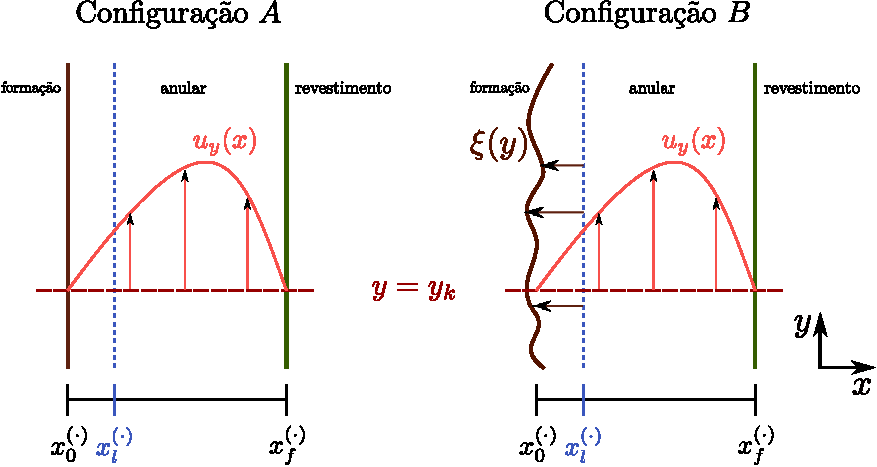
\includegraphics[scale=.8]{img/eta-esquema.pdf}
	\caption{Esquema representativo para cálculo de vazões nas configurações de poço não erodido ($A$) e poço erodido ($B$). Fonte: Autor.}
	\label{fig:eta-esquema}
\end{figure}

No segmento $[x_0^E,x_f^E]$ ($[x_0^D,x_f^D]$), escolhemos $x_l^E$ ($x_l^D$) como um ponto que particiona a porção anular esquerda em dois subsegmentos
tais que $[x_0^E,x_f^E]$ = $[x_0^E,x_l^E] \cup (x_l^E,x_f^E]$ ($[x_0^D,x_f^D]$ = $[x_0^D,x_l^D] \cup (x_l^D,x_f^D]$), onde $l$ indica que $x_l^E$ ($x_l^D$) está afastado de
$x_f^E$ ($x_f^D$) aproximadamente por um comprimento de $l$\% da largura da porção anular esquerda (direita).

Definimos
\begin{eqnarray}
    Q_p^{(q)}(y_k) &=& \int_{x_0^q}^{x_f^q} u_y(x) \, dx \, \Bigg|_{y = y_k}, \ \ \ q = D,E \ \ \text{e} \label{eq:vazaoA}\\
    Q_{p,l}^{(q)}(y_k) &=& \int_{x_l^q}^{x_f^q} u_y(x) \, dx \, \Bigg|_{y = y_k}, \ \ \ q = D,E, \label{eq:vazaoB}
\end{eqnarray}
respectivamente, como a \emph{vazão planar total na porção anular $q$} e a \emph{vazão planar percentual na porção anular $q$} na configuração $p$ à profundidade $y = y_k$. Isto é, tais quantidades representam medidas da frente de propagação do escoamento ao longo da direção $y$, levando em conta a variação da componente $u_y$ da velocidade sobre o corte transversal (direção $x$). Quando $p = A$, as quantidades referem-se ao caso de poço não erodido; quando $p = B$, ao caso de poço erodido.

A partir das Eqs. \eqref{eq:vazaoA} e \eqref{eq:vazaoB}, definimos
\begin{equation}
    %\eta_p^{(q)}(y_k) = \dfrac{Q_p^{(q)}(y_k) - Q_{p,l}^{(q)}(y_k)}{Q^{(q)}(y_k)}, \ \ p = A,B
    \eta_l^{(q)}(y_k) = \dfrac{Q_{B,l}^{(q)}(y_k)}{Q_{A,l}^{(q)}(y_k)} \times 100\%, \ \ q = D,E
\end{equation}
como o \emph{coeficiente de eficiência de varrido efetivo a $l\%$ do revestimento} na porção anular $q$, de maneira que
\begin{equation}
    %\eta^{(q)}(y_k) = \dfrac{\eta_B^{(q)}(y_k)}{\eta_A^{(q)}(y_k)} \times 100\%
    \eta^{(q)}(y_k) = \dfrac{Q_{B}^{(q)}(y_k)}{Q_{A}^{(q)}(y_k)} \times 100\%, \ \ q = D,E
\end{equation}
é o \emph{coeficiente de eficiência de varrido total} na porção anular $q$ para a profundidade $y_k$. Nesses termos, à medida que $\eta_l^{(q)}(y_k)$ ($\eta^{(q)}(y_k)$) tende a 100\%, o efeito das erosões sobre a propagação do escoamento é praticamente desprezível; opostamente, à medida que tende a 0\%, esse efeito é considerável.

Ambos os coeficientes usam a configuração não erodida como modelo de referência para a configuração erodida, permitindo, dessa maneira, a quantificação da influência das erosões na perda de vazão planar. Entretanto, o coeficiente de eficiência de varrido efetivo captura essa influência de modo indireto através da alteração detectada no escoamento apenas na porção livre do anular. Já o coeficiente de eficiência de varrido total mede a influência diretamente.


%Este parâmetro é obtido pela equação $\eta = \frac{Q - Q{limp}}{Q_{limp}}$. Onde, $Q$ é a vazão no espaço anular e ${Q_{limp}}$ é a vazão no espaço anular sem os efeitos da parede e do revestimento, onde a velocidade é zero, como é detalhado mais adiante. 
    
%Este parâmetro é calculado para o lado esquerdo e direito individualmente e para 3 níveis de profundidade distintas das geometrias.
    
%Inicialmente é utilizado o programa Paraview para processar os dados da simulação numérica e extrair o arquivo csv que possui os dados da última iteração, um arquivo para cada nível de profundidade definido através da ferramenta plotoverline no mesmo programa. Esse arquivo pode ser exportado, após aplicar o plotoverline no nível desejado, na opção Save Data.
    
%Após isso, é implementado um código em python para leitura e processamento do arquivo CSV com o foco em calcular o parâmetro de limpeza desejado. Para fins didáticos, será detalhado o funcionamento básico do código a seguir.
    
%A linha 1 é a leitura do arquivo de dados do perfil de velocidade em CSV. Há dados em $nan$ que provêm dos pontos que não intersectam a malha, portanto faz-se necessário limpar o dataframe e resetar o index, linha 2.
    
%    \begin{lstlisting}
%    	df = pd.read_csv('linha11-y240.csv')
%    	df = df.dropna().reset_index(drop=True)
%    \end{lstlisting}
    
%A linha 1 do cód. a seguir é a componente de velocidade na direção $x$ e a linha do 2 é a componente de velocidade na direção $y$. v é o modulo da velocidade. x é o eixo x.
    
 %   \begin{lstlisting}
 %   	vx = df['f_24:0']
 %   	vy = df['f_24:1']
 %   	v = np.sqrt(vx**2 + vy**2).values
 %   	x = df['Points:0'].values
 %   \end{lstlisting}
    
%O cód. a seguir plota o perfil de velocidade em todo o eixo x
    
 %   \begin{lstlisting}
%    	plt.plot(x,v)
 %   \end{lstlisting}
    
%    \begin{figure}[H]
 %   	\centering
 %   	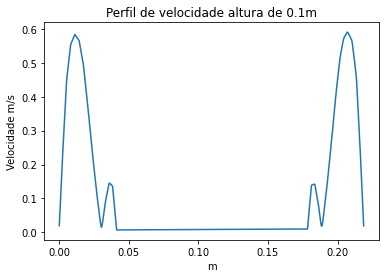
\includegraphics[scale=0.65]{img/perfil_vel/liso/perfil_velocidade_liso_100.png}
%	    \caption{Fonte: autor.}
 %   	\label{fig:perfil_velocidade_nivel_202}
 %   \end{figure}
    
%O cód. a seguir separa os dois lados onde o perfil de velocidade é diferente de zero, em outras palavras, o espaço anular esquerdo e o espaço anular direito. A imagem \ref{fig:perfil_velocidade_202_esquerdo} mostra o perfil de velocidade do lado esquerdo
    
%    \begin{lstlisting}
%    	nao_nulo_esq = np.argwhere((x < 33)).flatten()
 %   	nao_nulo_dir = np.argwhere((x > 135)).flatten()
 %   \end{lstlisting}
    
 %   \begin{figure}[H]
 %   	\centering
 %   	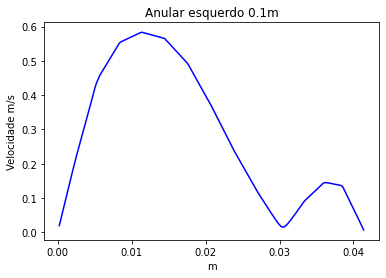
\includegraphics[scale=0.65]{img/perfil_vel/liso/perfil_velocidade_liso_esquerdo_100.png}
 %   	\caption{Fonte: autor.}
 %   	\label{fig:perfil_velocidade_202_esquerdo}
 %   \end{figure}
    
%A figura \ref{fig:/perfil_velocidade_202_esquerdo_delimitado} apresenta a eliminação do efeito de velocidade nula no contorno da formação.
    
 %   \begin{figure}[H]
 %   	\centering
 %   	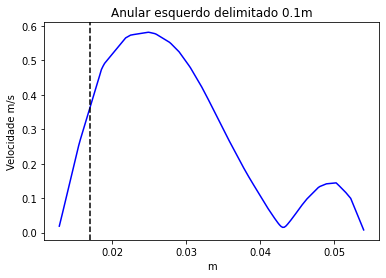
\includegraphics[scale=0.65]{img/perfil_vel/liso/perfil_velocidade_liso_esquerdo_delimitado_100.png}
%   	    \caption{Fonte: autor.}
%     	\label{fig:/perfil_velocidade_202_esquerdo_delimitado}
%     \end{figure}
    
% O cód. a seguir calcula a largura do espaço anular esquerdo e direito, $h_e$ e $h_d$ respectivamente
    
%     \begin{lstlisting}
%     	E = x[nao_nulo_esq]; D = x[nao_nulo_dir];
%     	h_e = np.max(E) - np.min(E)
%     	h_d = np.max(D) - np.min(D)
%     \end{lstlisting}
    
% O cód. a seguir calcula a área utilizando as equações $Qe = \int{he} ve dx$ e $Qd = \int{hd} vd dx$, do lado esquerdo e direito respectivamente. Para calcular é aplicado a integração numérica e regra do trapézio.
    
%     \begin{lstlisting}
%     	v_e = v[nao_nulo_esq]; v_d = v[nao_nulo_dir]
%     	Q_e = trapezoid(v_e)
%     	Q_d = trapezoid(v_d)
%     \end{lstlisting}
    
% Para calcular o parâmetro $\eta$ da eficiência de limpeza, é necessário "excluir" o efeito de velocidade nula no contorno do revestimento e da parede do poço. No espaço anular esquerdo o efeito do revestimento é do lado direto e o de parede é do lado esquerdo. No espaço anular direito, o efeito do revestimento é do lado esquerdo e o da parede é do lado direito. Foi adotado um percentual arbitrário de $10\%$ de ambos os lados do espaço anular para ser eliminado. Após isso, é necessário calcular a área no novo intervalo delimitado, ou seja, calcular a integral dos perfis de velocidade nos intervalos $[ha,hb]$ para obter $Q{limp}$
    
%     \begin{lstlisting}
%     	X = 0.1
%     	delta_e = X*h_e
%     	delta_d = X*h_d
%     	h_a = (delta_e,h_e - delta_e)
%     	h_b = (delta_d,h_d - delta_d) 
%     \end{lstlisting}
    
% Considerando apenas o lado esquerdo do espaço anular, o cálculo de $\eta_{e}$ é dado por  $\eta_{e} = \frac{Qe -	Q{limp_e}}{Q_{limp_e}}$ onde  $\eta_{e}$ é o parâmetro de limpeza do lado esquerdo, $Q{e}$ é a área do perfil de velocidade do lado esquerdo e $Q{limp_e}$ é a área do perfil de velocidade do lado esquerdo delimitado. O código a seguir representa esse cálculo 
%     \begin{lstlisting}
%     	n_e = (Q_e-Qlimpo_e)/Qlimpo_e
%     \end{lstlisting}
    
%     Esta análise acima é replicada para o lado direito do espaço anular.
